 \documentclass{article}
\usepackage{amsmath}
\usepackage{graphicx}
\usepackage{pgfplotstable}
\title{\LaTeX Assignments}
\author{Omkar Oak}
\date{24-11-22}
\begin{document}
\maketitle
\tableofcontents
\newpage
\section{Assignment 1: Data Structures and Algorithms}
\subsection{What is Data Structures}
A data structure is not only used for organizing the data. It is also used for processing, retrieving, and storing data. There are different basic and advanced types of data structures that are used in almost every program or software system that has been developed. So we must have good knowledge about data structures.
\subsection{Linear Data Structures}
Data structure in which data elements are arranged sequentially or linearly, where each element is attached to its previous and next adjacent elements, is called a linear data structure. 
\subsubsection{Static Data Structure}
Static data structure has a fixed memory size. It is easier to access the elements in a static data structure. 
 \subsubsection{Dynamic Data Structure}
In dynamic data structure, the size is not fixed. It can be randomly updated during the runtime which may be considered efficient concerning the memory (space) complexity of the code. 
\subsection{Non Linear Data Structures}
Data structures where data elements are not placed sequentially or linearly are called non-linear data structures. In a non-linear data structure, we can’t traverse all the elements in a single run only.
\newpage
\subsection{Arrays} 
\begin{itemize}
\item An array is a collection of items stored at contiguous memory locations. The idea is to store multiple items of the same type together.
\item This makes it easier to calculate the position of each element by simply adding an offset to a base value, i.e., the memory location of the first element of the array (generally denoted by the name of the array).
\end{itemize}
\subsection{Linked List}
A linked list is a linear data structure,in which the elements are not stored at contiguous memory locations.

\newpage
\begin{center}
	\section{Assignment 2: Mathematics Examination}
\end{center}
	\begin{center}
	\textbf{\Large College Of Engineering Pune}
	\end{center}
	\rule{\textwidth}{0.4pt}
	\begin{center}
	(MA-19002 Univariate Calculus)
	\end{center}
	Date: $23^{th}$ Nov 2022 \hspace{50 mm} Branch: Computer\\
	Program: S.Y.BTech \hspace{50 mm} Duration: 1 hour\\
	Semester: III \hspace{62 mm} Max marks: 20\\
	MIS No: 
	\begin{table}[h]
	\begin{tabular}{|l|c|c|c|c|c|c|c|c|r|}
	\hline
	 & & & & & & & & & \\
	\hline
	 \end{tabular}
	\end{table}
	\vspace{-6 mm}
	\section*{Instructions}
	\begin{itemize}
	\item Write your MIS number on paper.
	\item Unless otherwise mentioned symbols and notations have their usual standard meaning.
	\item Use of any kind of electronic device is NOT allowed.
	\item Any essential result, formula or theorem assumed for answering of questions must be clearly stated.
	\item Exam Duration: 1hr
	\item Maximum Marks: 20M
	\end{itemize}
	\hrule
	\begin{center}
\section*{Section I}
\end{center}
\subsection*{Question I}
1. Attempt the following questions:\\
a) Find the particular solution of the initial value problem: \hfill [CO2][{\bf 2}]
	
	\begin{align*}
	\tan x\frac{dy}{dx}&=y
	\\y(\frac{\pi}{2})&=(\frac{\pi}{2})
	\end{align*} 
\noindent b)Check the whether the following differential equation is exact or non-exact and justify your answer.\hfill [CO2][{\bf 2}]
	 \begin{equation*}
	 (1 + \ln xy)dx + (1 + \frac{x}{y})dy = 0
	\end{equation*}

2. Solve the following:
\begin{itemize}
 \item[a.)] $ 3x(xy - 2)dx + (x^3 + 2y)dy = 0 $\hfill [CO2][{\bf 2}]
 \item[b.)] $ (2\cos y +4x^2)dx - x \sin y = 0$\hfill [CO2][{\bf 3}]
\end{itemize}
\pagebreak
\vspace{-10 cm}
\subsection*{Question II}
1. Find eigenvalues and corresponding eigenvectors of A = 
	$\begin{bmatrix}
	2 & -1 \\ -1 & 2
	\end{bmatrix}$. Hence, find an orthogonal basis for $ R^2$
	\hfill [CO2][{\bf 2}]\\
2. Find the rank of matrix
	$\begin{bmatrix}
	8 & 6 & 4 & 1 & 3\\
	2 & 1 & -7 & 4 & 1\\	
	1 & 1 & -1 & 2 & 1\\
	1 & -1 & 2 & 0 & 0\\
	\end{bmatrix}$ 
	\hfill [CO3][{\bf 3}]\\\\
3. State whether the following differential equations are linear or non-linear, justify and solve:  \hfill [CO2][{\bf 4}]\\
	\begin{itemize}
	\item[(a)] $ xy' + 2y = \frac{e^{3x}}{x}, x>0$ with $y(1)=1+\frac{e^3}{3}$
	\item[(b)] $x^2y\frac{dy}{dx}-xy^2=1$
	\end{itemize}
4. Solve the Differential equation 
$\frac{dy}{dx} = \frac{tanx-x^2y-2y}{x^2-4x-1+e^x}$ \hfill [CO2][{\bf 2}] \\\\
5. Solve the following indefinite integral
$\int x \cos{x^2} dx$  \hfill [CO3][{\bf 3}]\\

\newpage
\section{Assignment 3}
\subsection{Adding Image}
	\begin{center}
	\begin{figure}[h]
	\caption{\begin{large}Japan\end{large}}
	\vspace{5 mm}
	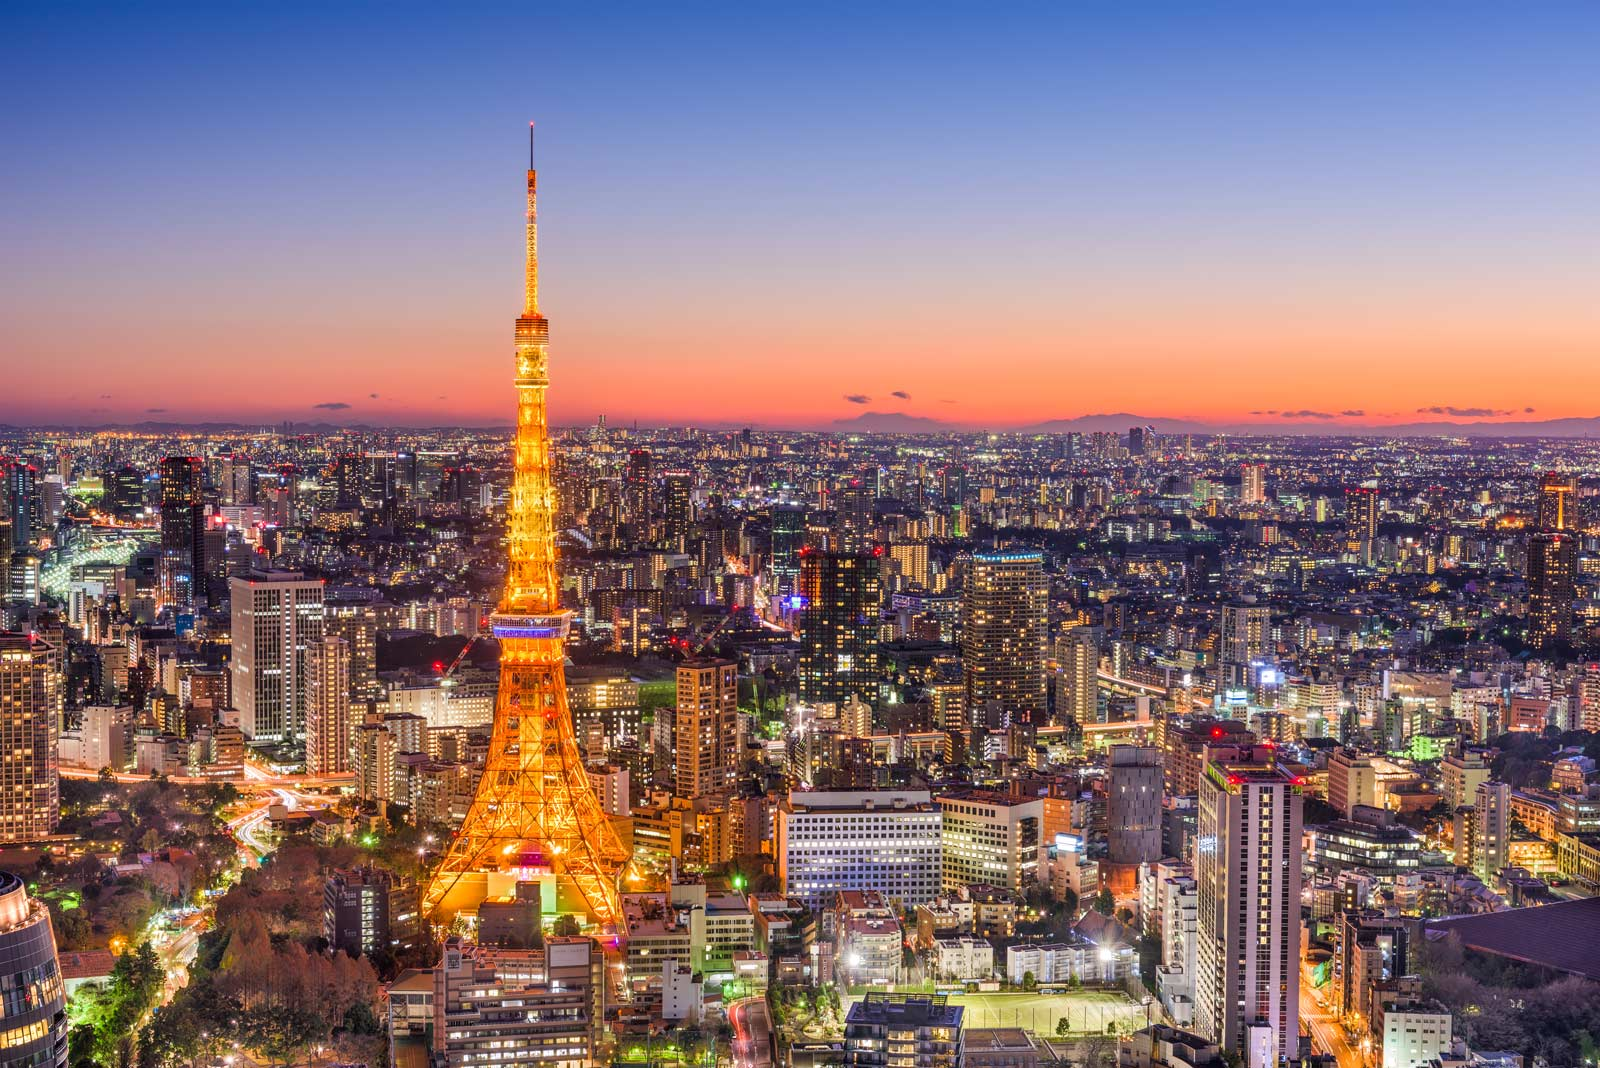
\includegraphics[width=13cm]{image1}
	\end{figure}
	\end{center}
	\subsection{Adding Table}
	\begin{table}[h]
	\begin{center}
	\caption{Cities of Japan}
	\vspace{5 mm}
	\begin{tabular}{|l|c|c|c|c|r|}
	\hline
	\textbf{Sr.No} & \textbf{City} & \textbf{District} & \textbf{Population}\\
	\hline
	1 & Tokyo & Tokyo City & 3,906,753,002 \\
	\hline
	2 & Osaka & Yamada ken & 3,206,453,779 \\
	\hline
	3 & Kyoto & Funigawa & 2,106,330,110\\
	\hline
	4 & Sapporo & Hokkaido & 1,020,030,000 \\
	\hline
	\end{tabular}
	\end{center}
	\end{table}
	\newpage
	
\section{Table Examples}
Study the following table and answer the questions based on it 
\cite{float}

\begin{table}[h] 
\begin{tabular}{|l|c|c|c|c|r|}
\hline
 & \multicolumn{4}{c}{Item of Expenditure} \\ \hline
Year & Salary & Fuel and Transport & Bonus & Interest of Loans & Taxes\\
 \hline
 1998 & 288 & 98 & 3.00 & 23.4 & 83 \\ 
  \hline
 1999 & 342 & 112 & 2.52 & 32.5 & 108 \\ 
  \hline
 2000 & 324 & 101 & 3.84 & 41.6 & 74 \\ 
 \hline
 2001 & 336 & 133 & 3.68 & 36.4 & 88 \\ 
 \hline
 2002 & 420 & 142 & 3.96 & 49.4 & 98 \\ 
 \hline
\end{tabular}
\caption{\label{Question I} Expenditures of a Company (in Lakh Rupees) per Annum Over the given Years.}
\end{table}


\begin{enumerate}
\item The total amount of bonus paid by the company during the given period is approximately what percent of the total amount of salary paid during this period?
\item Total expenditure on all these items in 1998 was approximately what percent of the total expenditure in 2002?
\item The total expenditure of the company over these items during the year 2000 is?
\item The ratio between the total expenditure on Taxes for all the years and the total expenditure on Fuel and Transport for all the years respectively is approximately?
\end{enumerate}


\begin{table}[h]
\begin{tabular}{|l|c|c|c|c|c|r|}
\hline
	& \multicolumn{6}{c}{Subject (Max. Marks)} \\ \hline
 Student & Maths	 & Chemistry	 & Physics & Geography & History & Comp Sci \\ \hline
Ayush	& 90 & 50 & 90 & 60 & 70 & 80 \\
Aman	    & 99 & 80 & 80 & 40 & 80 & 70 \\
Sajal	& 90 & 60 & 70 & 70 & 90 & 70 \\
Rohit	& 80 & 65 & 80 & 80 & 60 & 60 \\
Muskan	& 80 & 65 & 85 & 95 & 50 & 90 \\
Tanvi	& 70	 & 75 & 65 & 85 & 40 & 60 \\
Tarun	& 65 & 35 & 50 & 77 & 80	& 80 \\
\hline
\end{tabular}
\end{table}
\noindent \cite{theory} 
The above table gives the percentage of marks obtained by seven students in six different subjects in an examination. \\ 
\textit{The numbers in the brackets give the maximum marks in each subject.}

\begin{enumerate}
\item What are the average marks obtained by all the seven students in Physics? (rounded off to two digit after decimal)
\item The number of students who obtained 60\% and above marks in all subjects is?
\item What was the aggregate of marks obtained by Sajal in all the six subjects?
\item In which subject is the overall percentage the best?
\item What is the overall percentage of Tarun?
\end{enumerate}
\hrule

\section{Table from CSV}
\subsection*{Question I}
\begin{table}[h]
  \begin{center}
    \caption{Autogenerated table from .csv file.}
    \label{table1}
    \pgfplotstabletypeset[
	col sep=comma,
	columns = {Roll Number, Science, Computer, Maths, History}
]{data1.csv} % filename/path to file
  \end{center}
\end{table}
\begin{enumerate}
\item What is the total marks obtained by the student in history and computer together?
\item Who scored the lowest marks in all the subjects?
\item What is the median mark of the students in mathematics?
\item What is the range of marks obtained by the students in history?
\end{enumerate}
\pagebreak


\begin{thebibliography} {}
\bibitem{book} “Digital Design” M Morris Mano, 5th Edition, 2013, Pearson Education, ISBN-10: 0-13-277420-8 / ISBN-13: 978-0-13-277420-8
\bibitem {float} “Discrete Mathematics”, Lipschutz, Lipson, 2nd Edition, 1999, Tata McGraw-Hill, ISBN: 007 463710X
\bibitem{real} Real Number Symbol in LaTeX, $https://www.physicsread.com/latex-real-number/$
\bibitem {theory}“Theory of computer science”, E. V. Krishnamurthy, 2004, Affiliated East Press Publications, ISBN-10: 038791255X / ISBN-13: 978-0387912554.

\end{thebibliography}
\end{document}